\documentclass[12pt, border=12pt]{standalone}
\usepackage[utf8]{inputenc}
\usepackage[utf8]{vietnam}
\usepackage{amsmath,amsfonts,amssymb}
\usepackage{type1cm}
\usepackage{graphicx}
\usepackage{multirow}
\usepackage{multicol}
\usepackage{array}
\usepackage{comment}
\usepackage[unicode]{hyperref}
\usepackage{tikz}
\usepackage{color}
\usepackage[american,cuteinductors,smartlabels]{circuitikz}
\usetikzlibrary{arrows}
\usepackage{tikz}
\usetikzlibrary{calc,patterns,angles,quotes}
\usetikzlibrary{arrows, decorations.markings, calc, fadings, decorations.pathreplacing, patterns, decorations.pathmorphing, positioning}	
%\tikzstyle{every path}=[line width=1.2pt]

\tikzset{middlearrow/.style={
        decoration={markings,
            mark= at position 0.5 with {\arrow{#1}} ,
        },
        postaction={decorate}
    }
}
\begin{document}
	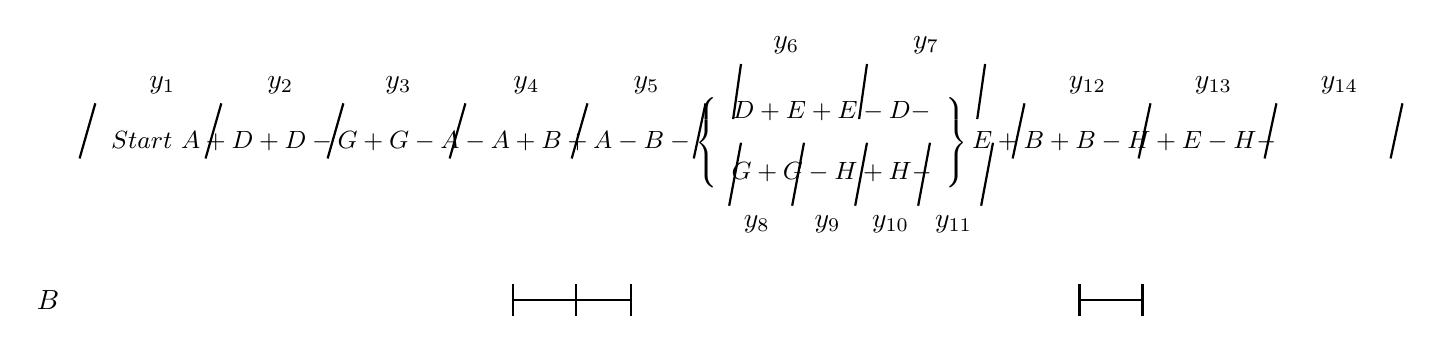
\begin{tikzpicture}[>=triangle 45]
		\draw (5,0) node {\small{$Start~A+D+D-G+G-A-A+B+A-B-\left\{\begin{array}{c}D+E+E-D-\\ \\G+G-H+H-\end{array}\right\}E+B+B-H+E-H-$}};								
		\draw[thick] (-2.6,0.5) -- (-2.8,-0.2);
		\draw[thick] (-1,0.5) -- (-1.2,-0.2); \draw (-1.75,0.5) node[above]{$y_1$};
						
		\draw[thick] (0.55,0.5) -- (0.35,-0.2); \draw (-0.25,0.5) node[above]{$y_2$};
						
		\draw[thick] (2.1,0.5) -- (1.9,-0.2); \draw (1.25,0.5) node[above]{$y_3$};
						
		\draw[thick] (3.65,0.5) -- (3.45,-0.2); \draw (2.875,0.5) node[above]{$y_4$};
						
		\draw[thick] (5.15,0.5) -- (5,-0.2); \draw (4.4,0.5) node[above]{$y_5$};
						
		\draw[thick] (5.6,1) -- (5.5,0.3);
		\draw[thick] (7.2,1) -- (7.1,0.3); \draw (6.175,1) node[above]{$y_6$};
						
		\draw[thick] (8.7,1) -- (8.6,0.3); \draw (7.95,1) node[above]{$y_7$};
							
		\draw[thick] (5.6,0) -- (5.45,-.8);
		\draw[thick] (6.4,0) -- (6.25,-.8); \draw (5.8,-.8) node[below]{$y_8$};
						
		\draw[thick] (7.2,0) -- (7.05,-.8); \draw (6.7,-0.8) node[below]{$y_9$};
						
		\draw[thick] (8,0) -- (7.85,-.8); \draw (7.5,-.8) node[below]{$y_{10}$};
						
		\draw[thick] (8.8,0) -- (8.65,-.8); \draw (8.3,-.8) node[below]{$y_{11}$};
						
		\draw[thick] (9.2,0.5) -- (9.05,-0.2);						
		\draw[thick] (10.8,0.5) -- (10.65,-0.2); \draw (10,.5) node[above]{$y_{12}$};
						
		\draw[thick] (12.4,0.5) -- (12.25,-0.2); \draw (11.6,.5) node[above]{$y_{13}$};
						
		\draw[thick] (14,0.5) -- (13.85,-0.2); \draw (13.2,.5) node[above]{$y_{14}$};
								
		\draw(-3.2,-2) node{$B$};
		\draw[thick] (2.7,-2) -- (3.5,-2); \draw[thick] (2.7,-1.8) -- (2.7,-2.2); \draw[thick] (3.5,-1.8) -- (3.5,-2.2);
								
		\draw[thick] (3.5,-2) -- (4.2,-2);  \draw[thick] (4.2,-1.8) -- (4.2,-2.2);
								
		\draw[thick] (9.9,-2) -- (10.7,-2); \draw[thick] (9.9,-1.8) -- (9.9,-2.2); \draw[thick] (10.7,-1.8) -- (10.7,-2.2);
	\end{tikzpicture}
\end{document}